\documentclass[twoside]{article}

% Packages required by doxygen
\usepackage{calc}
\usepackage{doxygen}
\usepackage{graphicx}
\usepackage[utf8]{inputenc}
\usepackage{makeidx}
\usepackage{multicol}
\usepackage{multirow}
\usepackage{textcomp}
\usepackage[table]{xcolor}

% NLS support packages
\usepackage{polski}
\usepackage[T1]{fontenc}

% Font selection
\usepackage[T1]{fontenc}
\usepackage{mathptmx}
\usepackage[scaled=.90]{helvet}
\usepackage{courier}
\usepackage{amssymb}
\usepackage{sectsty}
\renewcommand{\familydefault}{\sfdefault}
\allsectionsfont{%
  \fontseries{bc}\selectfont%
  \color{darkgray}%
}
\renewcommand{\DoxyLabelFont}{%
  \fontseries{bc}\selectfont%
  \color{darkgray}%
}

% Page & text layout
\usepackage{geometry}
\geometry{%
  a4paper,%
  top=2.5cm,%
  bottom=2.5cm,%
  left=2.5cm,%
  right=2.5cm%
}
\tolerance=750
\hfuzz=15pt
\hbadness=750
\setlength{\emergencystretch}{15pt}
\setlength{\parindent}{0cm}
\setlength{\parskip}{0.2cm}
\makeatletter
\renewcommand{\paragraph}{%
  \@startsection{paragraph}{4}{0ex}{-1.0ex}{1.0ex}{%
    \normalfont\normalsize\bfseries\SS@parafont%
  }%
}
\renewcommand{\subparagraph}{%
  \@startsection{subparagraph}{5}{0ex}{-1.0ex}{1.0ex}{%
    \normalfont\normalsize\bfseries\SS@subparafont%
  }%
}
\makeatother

% Headers & footers
\usepackage{fancyhdr}
\pagestyle{fancyplain}
\fancyhead[LE]{\fancyplain{}{\bfseries\thepage}}
\fancyhead[CE]{\fancyplain{}{}}
\fancyhead[RE]{\fancyplain{}{\bfseries\leftmark}}
\fancyhead[LO]{\fancyplain{}{\bfseries\rightmark}}
\fancyhead[CO]{\fancyplain{}{}}
\fancyhead[RO]{\fancyplain{}{\bfseries\thepage}}
\fancyfoot[LE]{\fancyplain{}{}}
\fancyfoot[CE]{\fancyplain{}{}}
\fancyfoot[RE]{\fancyplain{}{\bfseries\scriptsize Wygenerowano Śr, 28 maj 2014 20:34:16 dla Problem plecakowy programem Doxygen }}
\fancyfoot[LO]{\fancyplain{}{\bfseries\scriptsize Wygenerowano Śr, 28 maj 2014 20:34:16 dla Problem plecakowy programem Doxygen }}
\fancyfoot[CO]{\fancyplain{}{}}
\fancyfoot[RO]{\fancyplain{}{}}
\renewcommand{\footrulewidth}{0.4pt}
\renewcommand{\sectionmark}[1]{%
  \markright{\thesection\ #1}%
}

% Indices & bibliography
\usepackage{natbib}
\usepackage[titles]{tocloft}
\setcounter{tocdepth}{3}
\setcounter{secnumdepth}{5}
\makeindex

% Hyperlinks (required, but should be loaded last)
\usepackage{ifpdf}
\ifpdf
  \usepackage[pdftex,pagebackref=true]{hyperref}
\else
  \usepackage[ps2pdf,pagebackref=true]{hyperref}
\fi
\hypersetup{%
  colorlinks=true,%
  linkcolor=blue,%
  citecolor=blue,%
  unicode%
}

% Custom commands
\newcommand{\clearemptydoublepage}{%
  \newpage{\pagestyle{empty}\cleardoublepage}%
}


%===== C O N T E N T S =====

\begin{document}

% Titlepage & ToC
\hypersetup{pageanchor=false}
\pagenumbering{roman}
\begin{titlepage}
\vspace*{7cm}
\begin{center}%
{\Large Problem plecakowy }\\
\vspace*{1cm}
{\large Wygenerowano przez Doxygen 1.8.4}\\
\vspace*{0.5cm}
{\small Śr, 28 maj 2014 20:34:16}\\
\end{center}
\end{titlepage}
\tableofcontents
\pagenumbering{arabic}
\hypersetup{pageanchor=true}

%--- Begin generated contents ---
\section{Problem plecakowy}
\label{index}\hypertarget{index}{}\hypertarget{index_opis}{}\subsection{Opis programu}\label{index_opis}
Program struktury wykonuje pomiaru czasu wykonania algorytmu wypelniania jednej z czterech opcji\-: \par
\par
 {\bfseries S\-T\-O\-S}\par
 Sposob wywolania\-: {\itshape {\ttfamily ./struktury stack \mbox{[}rozmiar problemu\mbox{]} \mbox{[}ilosc powtorzen\mbox{]}}}\par
 Wykonuje podstawowe operacje na stosie. W przypadku przekroczenia rozmiaru tablicy zwieksza jej rozmiar o 1.\par


{\bfseries S\-T\-O\-S2}\par
 Sposob wywolania\-: {\itshape {\ttfamily ./struktury stack2 \mbox{[}rozmiar problemu\mbox{]} \mbox{[}ilosc powtorzen\mbox{]}}}\par
 Wykonuje podstawowe operacje na stosie. W przypadku przekroczenia rozmiaru tablicy zwieksza jej rozmiar 2 razy.\par


{\bfseries S\-T\-O\-S N\-A L\-I\-S\-C\-I\-E}\par
 Sposob wywolania\-: {\itshape {\ttfamily ./struktury stonlist \mbox{[}rozmiar problemu\mbox{]} \mbox{[}ilosc powtorzen\mbox{]}}}\par
 Wykonuje podstawowe operacje stosu na liscie.\par


{\bfseries K\-O\-L\-E\-J\-K\-A}\par
 Sposob wywolania\-: {\itshape {\ttfamily ./struktury queue \mbox{[}rozmiar problemu\mbox{]} \mbox{[}ilosc powtorzen\mbox{]}}}\par
 Wykonuje podstawowe operacje na kolejce (liscie jednokierunkowej).\par
\par
\hypertarget{index_autor}{}\subsection{Autor}\label{index_autor}
Program wykonala\-: Agnieszka Wisniewska, nr albumu\-: 200 466 
\section{Indeks hierarchiczny}
\subsection{Hierarchia klas}
Ta lista dziedziczenia posortowana jest z grubsza, choć nie całkowicie, alfabetycznie\-:\begin{DoxyCompactList}
\item \contentsline{section}{Item}{\pageref{class_item}}{}
\item vector\begin{DoxyCompactList}
\item \contentsline{section}{Itemlist}{\pageref{class_itemlist}}{}
\begin{DoxyCompactList}
\item \contentsline{section}{Suitcase}{\pageref{class_suitcase}}{}
\end{DoxyCompactList}
\end{DoxyCompactList}
\end{DoxyCompactList}

\section{Indeks klas}
\subsection{Lista klas}
Tutaj znajdują się klasy, struktury, unie i interfejsy wraz z ich krótkimi opisami\-:\begin{DoxyCompactList}
\item\contentsline{section}{\hyperlink{class_aarray}{Aarray$<$ Value $>$} }{\pageref{class_aarray}}{}
\item\contentsline{section}{\hyperlink{struct_aarray_1_1_pair}{Aarray$<$ Value $>$\-::\-Pair} }{\pageref{struct_aarray_1_1_pair}}{}
\end{DoxyCompactList}

\section{Indeks plików}
\subsection{Lista plików}
Tutaj znajduje się lista wszystkich plików z ich krótkimi opisami\-:\begin{DoxyCompactList}
\item\contentsline{section}{\hyperlink{array_8hh}{array.\-hh} \\*Plik zawiera definicje szablonu klasy \hyperlink{class_array}{Array} }{\pageref{array_8hh}}{}
\item\contentsline{section}{\hyperlink{benchmark_8cpp}{benchmark.\-cpp} \\*Plik zawiera implementacje klasy \hyperlink{class_benchmark}{Benchmark} }{\pageref{benchmark_8cpp}}{}
\item\contentsline{section}{\hyperlink{benchmark_8hh}{benchmark.\-hh} \\*Plik zawiera definicje klasy \hyperlink{class_benchmark}{Benchmark} oraz typu sorting\-Type }{\pageref{benchmark_8hh}}{}
\item\contentsline{section}{\hyperlink{heap_8hh}{heap.\-hh} }{\pageref{heap_8hh}}{}
\item\contentsline{section}{\hyperlink{main_8cpp}{main.\-cpp} \\*Plik zawiera glowna funkcje programu }{\pageref{main_8cpp}}{}
\item\contentsline{section}{\hyperlink{merge_8hh}{merge.\-hh} }{\pageref{merge_8hh}}{}
\item\contentsline{section}{\hyperlink{quicksort_8hh}{quicksort.\-hh} }{\pageref{quicksort_8hh}}{}
\end{DoxyCompactList}

\section{Dokumentacja klas}
\hypertarget{class_item}{\subsection{Dokumentacja klasy Item}
\label{class_item}\index{Item@{Item}}
}


{\ttfamily \#include $<$item.\-hh$>$}

\subsubsection*{Metody publiczne}
\begin{DoxyCompactItemize}
\item 
std\-::string \hyperlink{class_item_a97d9d20c9b42b9696be110c14897858c}{Get\-Name} () const 
\begin{DoxyCompactList}\small\item\em Funkcja pobierająca nazwę przedmiotu. \end{DoxyCompactList}\item 
int \hyperlink{class_item_a894a58fc7e4f82071babddc460a650b9}{Get\-Weight} () const 
\begin{DoxyCompactList}\small\item\em Funkcja pobierająca wagę przedmiotu. \end{DoxyCompactList}\item 
int \hyperlink{class_item_a0ccf2b4569f86a0c2ee55651042e581f}{Get\-Value} () const 
\begin{DoxyCompactList}\small\item\em Funkcja pobierająca wartość przedmiotu. \end{DoxyCompactList}\item 
float \hyperlink{class_item_a704556451d8c68a1c9c10d16fb407d56}{Get\-Value\-Per\-Weigt} () const 
\begin{DoxyCompactList}\small\item\em Funkcja pobierająca warość przedmiotu na 1 g. \end{DoxyCompactList}\item 
\hyperlink{class_item_a014bd03374db1413e4e154a6b82dadbb}{Item} (std\-::string i\-Name, int i\-Weight, int i\-Value)
\begin{DoxyCompactList}\small\item\em Konstruktor parametyczny klasy \hyperlink{class_item}{Item}. \end{DoxyCompactList}\end{DoxyCompactItemize}
\subsubsection*{Atrybuty prywatne}
\begin{DoxyCompactItemize}
\item 
std\-::string \hyperlink{class_item_a7d8799886dca624982c8af6887adf916}{Item\-Name}
\item 
int \hyperlink{class_item_ad7b5016b5e5b378559b138dea750d92b}{Item\-Weight}
\item 
int \hyperlink{class_item_ac6060c04d812737e6a0b57d593c6be98}{Item\-Value}
\end{DoxyCompactItemize}


\subsubsection{Dokumentacja konstruktora i destruktora}
\hypertarget{class_item_a014bd03374db1413e4e154a6b82dadbb}{\index{Item@{Item}!Item@{Item}}
\index{Item@{Item}!Item@{Item}}
\paragraph[{Item}]{\setlength{\rightskip}{0pt plus 5cm}Item\-::\-Item (
\begin{DoxyParamCaption}
\item[{std\-::string}]{i\-Name, }
\item[{int}]{i\-Weight, }
\item[{int}]{i\-Value}
\end{DoxyParamCaption}
)}}\label{class_item_a014bd03374db1413e4e154a6b82dadbb}


Konstruktor parametyczny klasy \hyperlink{class_item}{Item}. 



\subsubsection{Dokumentacja funkcji składowych}
\hypertarget{class_item_a97d9d20c9b42b9696be110c14897858c}{\index{Item@{Item}!Get\-Name@{Get\-Name}}
\index{Get\-Name@{Get\-Name}!Item@{Item}}
\paragraph[{Get\-Name}]{\setlength{\rightskip}{0pt plus 5cm}std\-::string Item\-::\-Get\-Name (
\begin{DoxyParamCaption}
{}
\end{DoxyParamCaption}
) const\hspace{0.3cm}{\ttfamily [inline]}}}\label{class_item_a97d9d20c9b42b9696be110c14897858c}


Funkcja pobierająca nazwę przedmiotu. 

\begin{DoxyReturn}{Zwraca}
nazwę przedmiotu 
\end{DoxyReturn}
\hypertarget{class_item_a0ccf2b4569f86a0c2ee55651042e581f}{\index{Item@{Item}!Get\-Value@{Get\-Value}}
\index{Get\-Value@{Get\-Value}!Item@{Item}}
\paragraph[{Get\-Value}]{\setlength{\rightskip}{0pt plus 5cm}int Item\-::\-Get\-Value (
\begin{DoxyParamCaption}
{}
\end{DoxyParamCaption}
) const\hspace{0.3cm}{\ttfamily [inline]}}}\label{class_item_a0ccf2b4569f86a0c2ee55651042e581f}


Funkcja pobierająca wartość przedmiotu. 

\begin{DoxyReturn}{Zwraca}
wartość przedmiotu w złotówkach 
\end{DoxyReturn}
\hypertarget{class_item_a704556451d8c68a1c9c10d16fb407d56}{\index{Item@{Item}!Get\-Value\-Per\-Weigt@{Get\-Value\-Per\-Weigt}}
\index{Get\-Value\-Per\-Weigt@{Get\-Value\-Per\-Weigt}!Item@{Item}}
\paragraph[{Get\-Value\-Per\-Weigt}]{\setlength{\rightskip}{0pt plus 5cm}float Item\-::\-Get\-Value\-Per\-Weigt (
\begin{DoxyParamCaption}
{}
\end{DoxyParamCaption}
) const\hspace{0.3cm}{\ttfamily [inline]}}}\label{class_item_a704556451d8c68a1c9c10d16fb407d56}


Funkcja pobierająca warość przedmiotu na 1 g. 

\begin{DoxyReturn}{Zwraca}
wartość przedmiotu na 1 g 
\end{DoxyReturn}
\hypertarget{class_item_a894a58fc7e4f82071babddc460a650b9}{\index{Item@{Item}!Get\-Weight@{Get\-Weight}}
\index{Get\-Weight@{Get\-Weight}!Item@{Item}}
\paragraph[{Get\-Weight}]{\setlength{\rightskip}{0pt plus 5cm}int Item\-::\-Get\-Weight (
\begin{DoxyParamCaption}
{}
\end{DoxyParamCaption}
) const\hspace{0.3cm}{\ttfamily [inline]}}}\label{class_item_a894a58fc7e4f82071babddc460a650b9}


Funkcja pobierająca wagę przedmiotu. 

\begin{DoxyReturn}{Zwraca}
waga przedmiotu w gramach 
\end{DoxyReturn}


\subsubsection{Dokumentacja atrybutów składowych}
\hypertarget{class_item_a7d8799886dca624982c8af6887adf916}{\index{Item@{Item}!Item\-Name@{Item\-Name}}
\index{Item\-Name@{Item\-Name}!Item@{Item}}
\paragraph[{Item\-Name}]{\setlength{\rightskip}{0pt plus 5cm}std\-::string Item\-::\-Item\-Name\hspace{0.3cm}{\ttfamily [private]}}}\label{class_item_a7d8799886dca624982c8af6887adf916}
\hypertarget{class_item_ac6060c04d812737e6a0b57d593c6be98}{\index{Item@{Item}!Item\-Value@{Item\-Value}}
\index{Item\-Value@{Item\-Value}!Item@{Item}}
\paragraph[{Item\-Value}]{\setlength{\rightskip}{0pt plus 5cm}int Item\-::\-Item\-Value\hspace{0.3cm}{\ttfamily [private]}}}\label{class_item_ac6060c04d812737e6a0b57d593c6be98}
\hypertarget{class_item_ad7b5016b5e5b378559b138dea750d92b}{\index{Item@{Item}!Item\-Weight@{Item\-Weight}}
\index{Item\-Weight@{Item\-Weight}!Item@{Item}}
\paragraph[{Item\-Weight}]{\setlength{\rightskip}{0pt plus 5cm}int Item\-::\-Item\-Weight\hspace{0.3cm}{\ttfamily [private]}}}\label{class_item_ad7b5016b5e5b378559b138dea750d92b}


Dokumentacja dla tej klasy została wygenerowana z plików\-:\begin{DoxyCompactItemize}
\item 
\hyperlink{item_8hh}{item.\-hh}\item 
\hyperlink{item_8cpp}{item.\-cpp}\end{DoxyCompactItemize}

\hypertarget{class_itemlist}{\subsection{Dokumentacja klasy Itemlist}
\label{class_itemlist}\index{Itemlist@{Itemlist}}
}


{\ttfamily \#include $<$itemlist.\-hh$>$}

Diagram dziedziczenia dla Itemlist\begin{figure}[H]
\begin{center}
\leavevmode
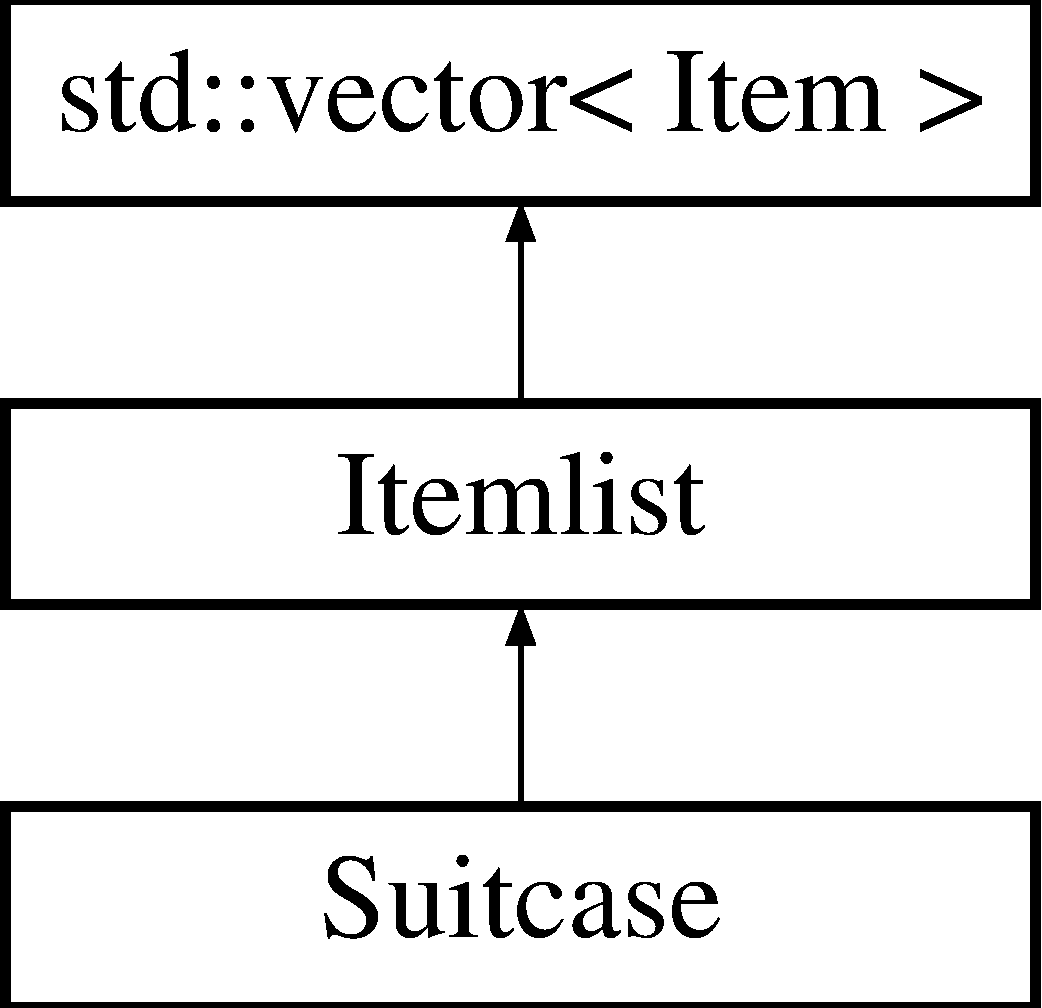
\includegraphics[height=3.000000cm]{class_itemlist}
\end{center}
\end{figure}
\subsubsection*{Metody publiczne}
\begin{DoxyCompactItemize}
\item 
bool \hyperlink{class_itemlist_a02210809223eb5fa5b5a064d6e89f4bc}{Load} (char $\ast$File\-Name)
\begin{DoxyCompactList}\small\item\em Funkcja wczytująca dane z pliku. \end{DoxyCompactList}\item 
void \hyperlink{class_itemlist_a7e9f18a1cd7f8a868aa0ff6389cfd3f0}{Show} ()
\begin{DoxyCompactList}\small\item\em Funkcja pomocnicza, wyświetlająca listę przedmiotów. \end{DoxyCompactList}\end{DoxyCompactItemize}


\subsubsection{Dokumentacja funkcji składowych}
\hypertarget{class_itemlist_a02210809223eb5fa5b5a064d6e89f4bc}{\index{Itemlist@{Itemlist}!Load@{Load}}
\index{Load@{Load}!Itemlist@{Itemlist}}
\paragraph[{Load}]{\setlength{\rightskip}{0pt plus 5cm}bool Itemlist\-::\-Load (
\begin{DoxyParamCaption}
\item[{char $\ast$}]{File\-Name}
\end{DoxyParamCaption}
)}}\label{class_itemlist_a02210809223eb5fa5b5a064d6e89f4bc}


Funkcja wczytująca dane z pliku. 

\begin{DoxyReturn}{Zwraca}
true , gdy plik zostanie wczytany poprawnie 

false , gdy przy wczytywaniu pliku wystąpi błąd 
\end{DoxyReturn}
\hypertarget{class_itemlist_a7e9f18a1cd7f8a868aa0ff6389cfd3f0}{\index{Itemlist@{Itemlist}!Show@{Show}}
\index{Show@{Show}!Itemlist@{Itemlist}}
\paragraph[{Show}]{\setlength{\rightskip}{0pt plus 5cm}void Itemlist\-::\-Show (
\begin{DoxyParamCaption}
{}
\end{DoxyParamCaption}
)}}\label{class_itemlist_a7e9f18a1cd7f8a868aa0ff6389cfd3f0}


Funkcja pomocnicza, wyświetlająca listę przedmiotów. 



Dokumentacja dla tej klasy została wygenerowana z plików\-:\begin{DoxyCompactItemize}
\item 
\hyperlink{itemlist_8hh}{itemlist.\-hh}\item 
\hyperlink{itemlist_8cpp}{itemlist.\-cpp}\end{DoxyCompactItemize}

\hypertarget{class_suitcase}{\subsection{Dokumentacja klasy Suitcase}
\label{class_suitcase}\index{Suitcase@{Suitcase}}
}


{\ttfamily \#include $<$suitcase.\-hh$>$}

Diagram dziedziczenia dla Suitcase\begin{figure}[H]
\begin{center}
\leavevmode
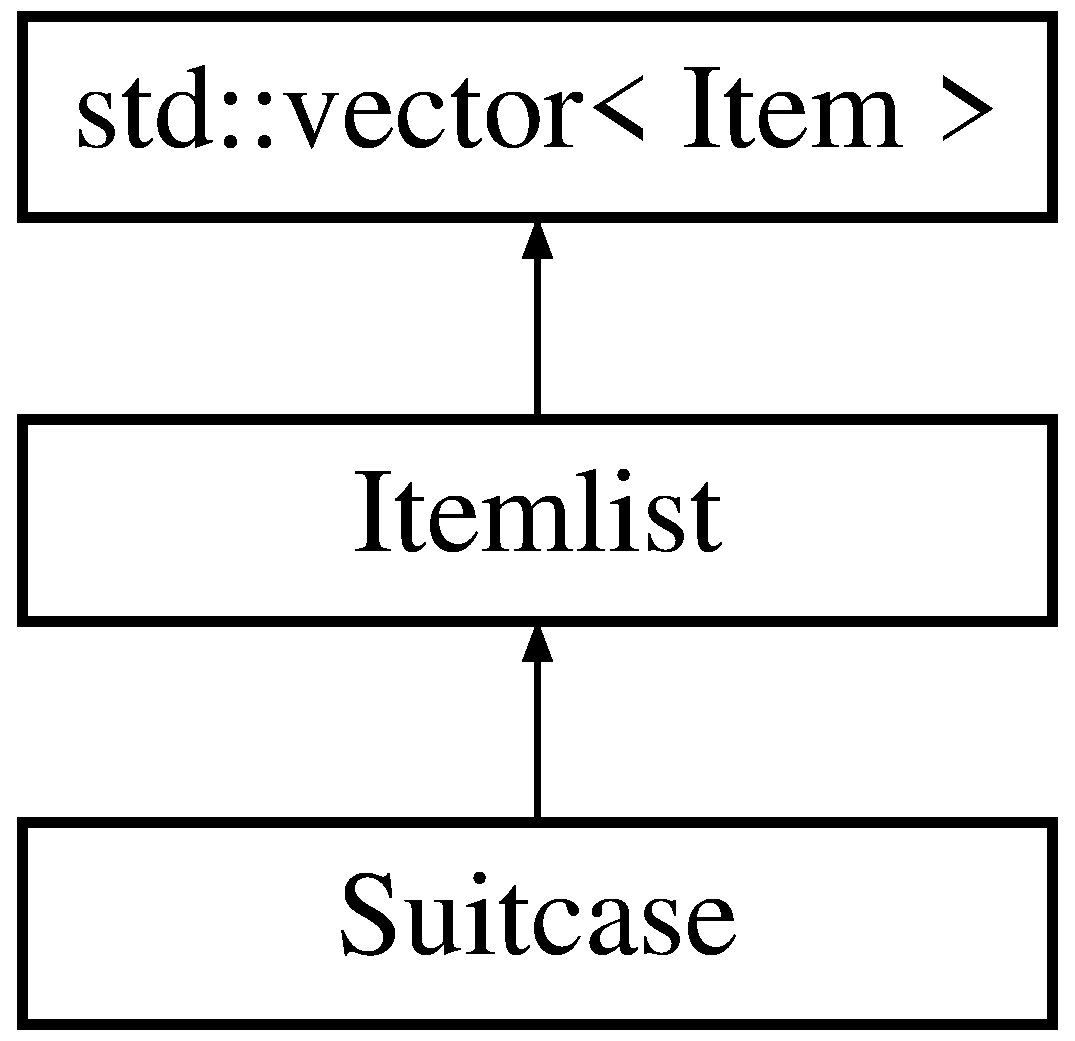
\includegraphics[height=3.000000cm]{class_suitcase}
\end{center}
\end{figure}
\subsubsection*{Metody publiczne}
\begin{DoxyCompactItemize}
\item 
\hyperlink{class_suitcase_a26538ae7fc5924073ccd21981c4e2ee3}{Suitcase} (int i\-Weight\-Limit)
\begin{DoxyCompactList}\small\item\em Konstruktor klasy \hyperlink{class_suitcase}{Suitcase}. \end{DoxyCompactList}\item 
bool \hyperlink{class_suitcase_af79ee9b926fd7043d67cf8d80d872371}{Put\-In} (const \hyperlink{class_item}{Item} item)
\begin{DoxyCompactList}\small\item\em Funkcja dodająca przedmiot do walizki. \end{DoxyCompactList}\item 
int \hyperlink{class_suitcase_a7b48ae73ae1f9a08a9c17d0a1df02bd6}{Weight\-Left} ()
\begin{DoxyCompactList}\small\item\em Funkcja zwracająca pozsotałą masę do wypełnienia walizki. \end{DoxyCompactList}\item 
void \hyperlink{class_suitcase_ad671edca529a637145bfa2de1f491373}{Clear} ()
\begin{DoxyCompactList}\small\item\em Funkcja opróżniająca walizkę \end{DoxyCompactList}\item 
int \hyperlink{class_suitcase_a7a35f87239170b275518f2e4211fbbb7}{Worth} ()
\begin{DoxyCompactList}\small\item\em Funkcja zwracająca wartość przedmiotów znajdujących się w walizce. \end{DoxyCompactList}\end{DoxyCompactItemize}
\subsubsection*{Atrybuty prywatne}
\begin{DoxyCompactItemize}
\item 
int \hyperlink{class_suitcase_a7bc04635b9636279709ad3ff1f2281bd}{Weight\-Limit}
\item 
int \hyperlink{class_suitcase_a67dfe88f590b9985b436a813596f22e6}{Act\-Weight}
\item 
int \hyperlink{class_suitcase_a38f65d031935c37d82b9813d83accadd}{Act\-Value}
\end{DoxyCompactItemize}


\subsubsection{Dokumentacja konstruktora i destruktora}
\hypertarget{class_suitcase_a26538ae7fc5924073ccd21981c4e2ee3}{\index{Suitcase@{Suitcase}!Suitcase@{Suitcase}}
\index{Suitcase@{Suitcase}!Suitcase@{Suitcase}}
\paragraph[{Suitcase}]{\setlength{\rightskip}{0pt plus 5cm}Suitcase\-::\-Suitcase (
\begin{DoxyParamCaption}
\item[{int}]{i\-Weight\-Limit}
\end{DoxyParamCaption}
)}}\label{class_suitcase_a26538ae7fc5924073ccd21981c4e2ee3}


Konstruktor klasy \hyperlink{class_suitcase}{Suitcase}. 


\begin{DoxyParams}{Parametry}
{\em i\-Weight\-Limit} & maksymalna wartość wagowa \\
\hline
\end{DoxyParams}


\subsubsection{Dokumentacja funkcji składowych}
\hypertarget{class_suitcase_ad671edca529a637145bfa2de1f491373}{\index{Suitcase@{Suitcase}!Clear@{Clear}}
\index{Clear@{Clear}!Suitcase@{Suitcase}}
\paragraph[{Clear}]{\setlength{\rightskip}{0pt plus 5cm}void Suitcase\-::\-Clear (
\begin{DoxyParamCaption}
{}
\end{DoxyParamCaption}
)}}\label{class_suitcase_ad671edca529a637145bfa2de1f491373}


Funkcja opróżniająca walizkę 

\hypertarget{class_suitcase_af79ee9b926fd7043d67cf8d80d872371}{\index{Suitcase@{Suitcase}!Put\-In@{Put\-In}}
\index{Put\-In@{Put\-In}!Suitcase@{Suitcase}}
\paragraph[{Put\-In}]{\setlength{\rightskip}{0pt plus 5cm}bool Suitcase\-::\-Put\-In (
\begin{DoxyParamCaption}
\item[{const {\bf Item}}]{item}
\end{DoxyParamCaption}
)}}\label{class_suitcase_af79ee9b926fd7043d67cf8d80d872371}


Funkcja dodająca przedmiot do walizki. 


\begin{DoxyParams}{Parametry}
{\em item} & obiekt klasy \hyperlink{class_item}{Item} \\
\hline
\end{DoxyParams}
\begin{DoxyReturn}{Zwraca}
true , gdy dodano obiekt do walizki 

false , gdy nie można dodać obiektu (np.\-: przekracza pozostałą wagę) 
\end{DoxyReturn}
\hypertarget{class_suitcase_a7b48ae73ae1f9a08a9c17d0a1df02bd6}{\index{Suitcase@{Suitcase}!Weight\-Left@{Weight\-Left}}
\index{Weight\-Left@{Weight\-Left}!Suitcase@{Suitcase}}
\paragraph[{Weight\-Left}]{\setlength{\rightskip}{0pt plus 5cm}int Suitcase\-::\-Weight\-Left (
\begin{DoxyParamCaption}
{}
\end{DoxyParamCaption}
)}}\label{class_suitcase_a7b48ae73ae1f9a08a9c17d0a1df02bd6}


Funkcja zwracająca pozsotałą masę do wypełnienia walizki. 

\begin{DoxyReturn}{Zwraca}
pozostała masa 
\end{DoxyReturn}
\hypertarget{class_suitcase_a7a35f87239170b275518f2e4211fbbb7}{\index{Suitcase@{Suitcase}!Worth@{Worth}}
\index{Worth@{Worth}!Suitcase@{Suitcase}}
\paragraph[{Worth}]{\setlength{\rightskip}{0pt plus 5cm}int Suitcase\-::\-Worth (
\begin{DoxyParamCaption}
{}
\end{DoxyParamCaption}
)}}\label{class_suitcase_a7a35f87239170b275518f2e4211fbbb7}


Funkcja zwracająca wartość przedmiotów znajdujących się w walizce. 

\begin{DoxyReturn}{Zwraca}
aktualna wartość przedmiotów w walizce 
\end{DoxyReturn}


\subsubsection{Dokumentacja atrybutów składowych}
\hypertarget{class_suitcase_a38f65d031935c37d82b9813d83accadd}{\index{Suitcase@{Suitcase}!Act\-Value@{Act\-Value}}
\index{Act\-Value@{Act\-Value}!Suitcase@{Suitcase}}
\paragraph[{Act\-Value}]{\setlength{\rightskip}{0pt plus 5cm}int Suitcase\-::\-Act\-Value\hspace{0.3cm}{\ttfamily [private]}}}\label{class_suitcase_a38f65d031935c37d82b9813d83accadd}
\hypertarget{class_suitcase_a67dfe88f590b9985b436a813596f22e6}{\index{Suitcase@{Suitcase}!Act\-Weight@{Act\-Weight}}
\index{Act\-Weight@{Act\-Weight}!Suitcase@{Suitcase}}
\paragraph[{Act\-Weight}]{\setlength{\rightskip}{0pt plus 5cm}int Suitcase\-::\-Act\-Weight\hspace{0.3cm}{\ttfamily [private]}}}\label{class_suitcase_a67dfe88f590b9985b436a813596f22e6}
\hypertarget{class_suitcase_a7bc04635b9636279709ad3ff1f2281bd}{\index{Suitcase@{Suitcase}!Weight\-Limit@{Weight\-Limit}}
\index{Weight\-Limit@{Weight\-Limit}!Suitcase@{Suitcase}}
\paragraph[{Weight\-Limit}]{\setlength{\rightskip}{0pt plus 5cm}int Suitcase\-::\-Weight\-Limit\hspace{0.3cm}{\ttfamily [private]}}}\label{class_suitcase_a7bc04635b9636279709ad3ff1f2281bd}


Dokumentacja dla tej klasy została wygenerowana z plików\-:\begin{DoxyCompactItemize}
\item 
\hyperlink{suitcase_8hh}{suitcase.\-hh}\item 
\hyperlink{suitcase_8cpp}{suitcase.\-cpp}\end{DoxyCompactItemize}

\section{Dokumentacja plików}
\hypertarget{item_8cpp}{\subsection{Dokumentacja pliku item.\-cpp}
\label{item_8cpp}\index{item.\-cpp@{item.\-cpp}}
}
{\ttfamily \#include \char`\"{}item.\-hh\char`\"{}}\\*


\subsubsection{Opis szczegółowy}
Plik zawierający implementacje funkcji klasy \hyperlink{class_item}{Item}. 
\hypertarget{item_8hh}{\subsection{Dokumentacja pliku item.\-hh}
\label{item_8hh}\index{item.\-hh@{item.\-hh}}
}


Plik zawierający metody oraz definicje klasy \hyperlink{class_item}{Item}.  


{\ttfamily \#include $<$string$>$}\\*
\subsubsection*{Komponenty}
\begin{DoxyCompactItemize}
\item 
class \hyperlink{class_item}{Item}
\end{DoxyCompactItemize}


\subsubsection{Opis szczegółowy}
Plik zawierający metody oraz definicje klasy \hyperlink{class_item}{Item}. 
\hypertarget{itemlist_8cpp}{\subsection{Dokumentacja pliku itemlist.\-cpp}
\label{itemlist_8cpp}\index{itemlist.\-cpp@{itemlist.\-cpp}}
}
{\ttfamily \#include \char`\"{}itemlist.\-hh\char`\"{}}\\*
{\ttfamily \#include $<$fstream$>$}\\*
{\ttfamily \#include $<$string$>$}\\*
{\ttfamily \#include $<$iostream$>$}\\*


\subsubsection{Opis szczegółowy}
Plik zawierający implementacje funkcji klasy \hyperlink{class_itemlist}{Itemlist}. 
\hypertarget{itemlist_8hh}{\subsection{Dokumentacja pliku itemlist.\-hh}
\label{itemlist_8hh}\index{itemlist.\-hh@{itemlist.\-hh}}
}


Plik zawierający metody oraz definicje klasy \hyperlink{class_itemlist}{Itemlist}.  


{\ttfamily \#include $<$vector$>$}\\*
{\ttfamily \#include $<$item.\-hh$>$}\\*
\subsubsection*{Komponenty}
\begin{DoxyCompactItemize}
\item 
class \hyperlink{class_itemlist}{Itemlist}
\end{DoxyCompactItemize}


\subsubsection{Opis szczegółowy}
Plik zawierający metody oraz definicje klasy \hyperlink{class_itemlist}{Itemlist}. 
\hypertarget{main_8cpp}{\subsection{Dokumentacja pliku main.\-cpp}
\label{main_8cpp}\index{main.\-cpp@{main.\-cpp}}
}
{\ttfamily \#include \char`\"{}itemlist.\-hh\char`\"{}}\\*
{\ttfamily \#include \char`\"{}suitcase.\-hh\char`\"{}}\\*
{\ttfamily \#include $<$iostream$>$}\\*
{\ttfamily \#include $<$cstdlib$>$}\\*
\subsubsection*{Funkcje}
\begin{DoxyCompactItemize}
\item 
int \hyperlink{main_8cpp_a3c04138a5bfe5d72780bb7e82a18e627}{main} (int argc, char $\ast$$\ast$argv)
\end{DoxyCompactItemize}


\subsubsection{Opis szczegółowy}
Plik zawierający główną funkcję programu. 

\subsubsection{Dokumentacja funkcji}
\hypertarget{main_8cpp_a3c04138a5bfe5d72780bb7e82a18e627}{\index{main.\-cpp@{main.\-cpp}!main@{main}}
\index{main@{main}!main.cpp@{main.\-cpp}}
\paragraph[{main}]{\setlength{\rightskip}{0pt plus 5cm}int main (
\begin{DoxyParamCaption}
\item[{int}]{argc, }
\item[{char $\ast$$\ast$}]{argv}
\end{DoxyParamCaption}
)}}\label{main_8cpp_a3c04138a5bfe5d72780bb7e82a18e627}

\hypertarget{mainpage_8dox}{\subsection{Dokumentacja pliku mainpage.\-dox}
\label{mainpage_8dox}\index{mainpage.\-dox@{mainpage.\-dox}}
}

\hypertarget{suitcase_8cpp}{\subsection{Dokumentacja pliku suitcase.\-cpp}
\label{suitcase_8cpp}\index{suitcase.\-cpp@{suitcase.\-cpp}}
}
{\ttfamily \#include \char`\"{}suitcase.\-hh\char`\"{}}\\*
{\ttfamily \#include $<$algorithm$>$}\\*
\subsubsection*{Funkcje}
\begin{DoxyCompactItemize}
\item 
bool \hyperlink{suitcase_8cpp_ac0e2271f3e1a79276dfe322e4c8f208d}{Compare\-By\-Value} (\hyperlink{class_item}{Item} item1, \hyperlink{class_item}{Item} item2)
\item 
void \hyperlink{suitcase_8cpp_a6ddaff0caa608ea223e157b69c733d42}{Knapsack} (\hyperlink{class_itemlist}{Itemlist} $\ast$item, \hyperlink{class_suitcase}{Suitcase} $\ast$suitcase)
\begin{DoxyCompactList}\small\item\em Funkcja pakująca rzeczy do walizki tak, aby ich wartość była jak największa, a waga nie została przekroczona. \end{DoxyCompactList}\end{DoxyCompactItemize}


\subsubsection{Opis szczegółowy}
Plik zawierający implementacje funkcji klasy \hyperlink{class_suitcase}{Suitcase}. 

\subsubsection{Dokumentacja funkcji}
\hypertarget{suitcase_8cpp_ac0e2271f3e1a79276dfe322e4c8f208d}{\index{suitcase.\-cpp@{suitcase.\-cpp}!Compare\-By\-Value@{Compare\-By\-Value}}
\index{Compare\-By\-Value@{Compare\-By\-Value}!suitcase.cpp@{suitcase.\-cpp}}
\paragraph[{Compare\-By\-Value}]{\setlength{\rightskip}{0pt plus 5cm}bool Compare\-By\-Value (
\begin{DoxyParamCaption}
\item[{{\bf Item}}]{item1, }
\item[{{\bf Item}}]{item2}
\end{DoxyParamCaption}
)}}\label{suitcase_8cpp_ac0e2271f3e1a79276dfe322e4c8f208d}
\hypertarget{suitcase_8cpp_a6ddaff0caa608ea223e157b69c733d42}{\index{suitcase.\-cpp@{suitcase.\-cpp}!Knapsack@{Knapsack}}
\index{Knapsack@{Knapsack}!suitcase.cpp@{suitcase.\-cpp}}
\paragraph[{Knapsack}]{\setlength{\rightskip}{0pt plus 5cm}void Knapsack (
\begin{DoxyParamCaption}
\item[{{\bf Itemlist} $\ast$}]{myitems, }
\item[{{\bf Suitcase} $\ast$}]{mysuitcase}
\end{DoxyParamCaption}
)}}\label{suitcase_8cpp_a6ddaff0caa608ea223e157b69c733d42}


Funkcja pakująca rzeczy do walizki tak, aby ich wartość była jak największa, a waga nie została przekroczona. 


\begin{DoxyParams}{Parametry}
{\em myitems} & wskaźnik na listę przedmiotów do zapakowania \\
\hline
{\em mysuitcase} & wskaźnik na walizkę do której będziemy pakować przedmioty \\
\hline
\end{DoxyParams}

\hypertarget{suitcase_8hh}{\subsection{Dokumentacja pliku suitcase.\-hh}
\label{suitcase_8hh}\index{suitcase.\-hh@{suitcase.\-hh}}
}


Plik zawierający metody oraz definicje klasy \hyperlink{class_suitcase}{Suitcase}.  


{\ttfamily \#include \char`\"{}itemlist.\-hh\char`\"{}}\\*
\subsubsection*{Komponenty}
\begin{DoxyCompactItemize}
\item 
class \hyperlink{class_suitcase}{Suitcase}
\end{DoxyCompactItemize}
\subsubsection*{Funkcje}
\begin{DoxyCompactItemize}
\item 
void \hyperlink{suitcase_8hh_a4ba16b1e7e4d4987ed40e3794085454a}{Knapsack} (\hyperlink{class_itemlist}{Itemlist} $\ast$myitems, \hyperlink{class_suitcase}{Suitcase} $\ast$mysuitcase)
\begin{DoxyCompactList}\small\item\em Funkcja pakująca rzeczy do walizki tak, aby ich wartość była jak największa, a waga nie została przekroczona. \end{DoxyCompactList}\end{DoxyCompactItemize}


\subsubsection{Opis szczegółowy}
Plik zawierający metody oraz definicje klasy \hyperlink{class_suitcase}{Suitcase}. 

\subsubsection{Dokumentacja funkcji}
\hypertarget{suitcase_8hh_a4ba16b1e7e4d4987ed40e3794085454a}{\index{suitcase.\-hh@{suitcase.\-hh}!Knapsack@{Knapsack}}
\index{Knapsack@{Knapsack}!suitcase.hh@{suitcase.\-hh}}
\paragraph[{Knapsack}]{\setlength{\rightskip}{0pt plus 5cm}void Knapsack (
\begin{DoxyParamCaption}
\item[{{\bf Itemlist} $\ast$}]{myitems, }
\item[{{\bf Suitcase} $\ast$}]{mysuitcase}
\end{DoxyParamCaption}
)}}\label{suitcase_8hh_a4ba16b1e7e4d4987ed40e3794085454a}


Funkcja pakująca rzeczy do walizki tak, aby ich wartość była jak największa, a waga nie została przekroczona. 


\begin{DoxyParams}{Parametry}
{\em myitems} & wskaźnik na listę przedmiotów do zapakowania \\
\hline
{\em mysuitcase} & wskaźnik na walizkę do której będziemy pakować przedmioty \\
\hline
\end{DoxyParams}

%--- End generated contents ---

% Index
\newpage
\phantomsection
\addcontentsline{toc}{part}{Indeks}
\printindex

\end{document}
